\documentclass[oneside,10pt,onecolumn]{waflreport}
% can use option mtpro 

\usepackage{graphicx}
\usepackage{rotating}
\usepackage{scalefnt}
\usepackage{bm}


\newlength\lengthfigure                  % declare a figure width unit
\setlength\lengthfigure{0.158\textwidth} % make the figure width unit scale with the textwidth
\renewcommand{\fontsizetable}{\footnotesize\scalefont{1.0}}
\renewcommand{\fontsizefigure}{\footnotesize}
\renewcommand{\vec}[1]{\bm{#1}}
\let\citen\cite
\setcounter{tocdepth}{3}
\newcommand{\mfd}{\displaystyle}
\newcommand{\Cp}{{C_{P}}}
\newcommand{\ie}{{\it i.e.}}
\newcommand{\pseudot}{\tau}
\newcommand{\ns}{{{n}_{\rm s}}}
\newcommand\frameeqn[1]{\fbox{$\displaystyle #1$}}
\newcommand{\ordi}{\; {\rm d}}
\newcommand{\alb}{\vspace{0.1cm}\\} % array line break
\newcommand{\Sda}{S_{{\rm d}A}}
\newcommand{\Schem}{S_{\rm chem}}
\newcommand{\Smhd}{S_{\rm MHD}}
\newcommand{\Sturb}{S_{\rm turb}}
\newcommand{\Bdipole}{B_{\rm d}}




\author{
  Bernard Parent
}

\email{
  parent@pnu.edu
}

\department{
  Dept. of Aerospace Engineering
}

\institution{
  Pusan National University
}

\title{
  Introduction to \LaTeX
}

\date{
  January 2010
}

%\setlength\nomenclaturelabelwidth{0.13\hsize}  % optional, default is 0.03\hsize
%\setlength\nomenclaturecolumnsep{0.09\hsize}  % optional, default is 0.06\hsize

\nomenclature{
  \begin{nomenclaturelist}{Roman symbols}
   \item[$\vec{A}$] origin of the magnet dipole moment
   \item[$A$]         cross-sectional area, $\rm m^2$
  \end{nomenclaturelist}


  \begin{nomenclaturelist}{Greek symbols}
   \item[$\alpha_{ij}$]  commonly used term in the diffusion matrix $K$
  \end{nomenclaturelist}


  \begin{nomenclaturelist}{Superscripts}
   \item[$\star$]    sum of turbulent and molecular diffusion
  \end{nomenclaturelist}

  \begin{nomenclaturelist}{Subscripts}
   \item[$t$]      turbulent
  \end{nomenclaturelist}
}


\abstract{
The goal of this report is to give examples of how to typeset mathematics using \LaTeX\ and how to include figures and tables within a document. 
}

\begin{document}
  \pagestyle{headings}
  \pagenumbering{arabic}
  \setcounter{page}{1}
%%  \maketitle
  \makewaflreporttitle
  \makeabstract
  \tableofcontents
  \makenomenclature
%%  \listoftables
%%  \listoffigures




























\section{Introduction and motivation}

There has been a substantial recent interest in how to
improve the performance of hypervelocity flight vehicles with MHD. One such application
is the bypass of the flow mechanical energy from the inlet to the nozzle (such as in
project AJAX \cite{aiaaconf:1996:gurijanov,aiaaconf:2001:kuranov} or
others \cite{aiaabook:2001:vatazhin,jpp:2001:litchford}).
By bypassing some of the flow mechanical energy around the combustor, it is hoped
that the flow velocity in the combustor can be reduced to subsonic speeds while
maintaining the maximum static temperature at the combustor entrance to a reasonable
value. However, to the author's knowledge, a numerical or experimental study of this MHD-ramjet
showing a benefit over the conventional ramjet (without energy bypass) has not yet
appeared in the open litterature. One of the goals of the present report is hence to
investigate on whether the flow can be slowed to subsonic speeds while maintaining
the temperature to below a certain limit through the use of MHD energy extraction.

Other
possible applications of MHD to hypersonic flight include the observed drag reduction
over blunt bodies when an external magnetic field is applied to a conducting incoming
flow (see Ref.\ \cite{aiaa:2002:shang} for instance), and the control of the shock positioning
in a scramjet inlet to achieve shock-on-lip condition over a relatively wide Mach number range
\cite{aiaaconf:2002:shneider} while keeping the geometry fixed.


There is also
a considerable interest in MHD as a means to generate electrical
power aboard a high-speed flight vehicle. The drastically high mechanical
energy of the flow at a high Mach number can be converted to electrical energy
through a MHD generator at the expense of a sudden reduction in flight speed.
Preliminary estimates show that a power
of hundreds of thousands of megawatts per cubic meter could be produced in such a way
\cite{aiaaconf:2002:thibodeaux}. The power
could then be used to feed a high-energy laser aimed at ground, air, or space targets. No
other known source of energy (except nuclear) could generate this type of power.

Yet other advantages of the presence of a weakly ionized flow in a hypersonic propulsion
device include the possible increase in mixing and ignition \cite{aiaaconf:2002:bocharov}
or the decrease in induction time of the burning
of a kerosene-air mixture \cite{aiaaconf:2002:klimov}. The latter is
particularly important to the possibility of using kerosene in small-size scramjets due
to the very high kerosene/air mixture induction time for burning as compared to a mixture
of hydrogen and air.


In this report, the WARP code \cite{jcp:2002:parent,aiaa:2002:parent}
is extended to the weakly-ionized MHD equations in order to simulate artificially
ionized flows in scramjets/shcramjets where an interaction with a strong external
magnetic field is present.

%%%%%%%%%%%%%%%%%%%%%%%%%%%%%%%%%%%%%%%%%%%%%%%%%%%%%%%%%%%%%%%%%%%%%%%%%%%%%%%%%%%%%%%%%%%%%%%%%%%%%%
%%%%%%%%%%%%%%%%%%%%%%%%%%%%%%%%%%%%%%%%%%%%%%%%%%%%%%%%%%%%%%%%%%%%%%%%%%%%%%%%%%%%%%%%%%%%%%%%%%%%%%
%%%%%%%%%%%%%%%%%%%%%%%%%%%%%%%%%%%%%%%%%%%%%%%%%%%%%%%%%%%%%%%%%%%%%%%%%%%%%%%%%%%%%%%%%%%%%%%%%%%%%%


\section{Quasi-one-dimensional perfect-gas flow}

This section is focused on studying the impact of the MHD source terms on the flow for the case
of quasi-one-dimensional formulation. This can be done numerically by trying out several
configurations, but this can also be done analytically, as is performed now.

\subsection{Governing equations}

%
Let's
first write down the steady-state quasi-one-dimensional MHD equations for a calorically and thermally
perfect gas, without any chemistry:
%
\begin{equation}
  \frac{\ordi}{\ordi x}
     \left[
      \begin{array}{@{}c@{}}
        A {\rho} q \alb
        A {\rho} q^2 +  A P\alb
        A {\rho} q \left(e+q^2/2\right)+ A q P \alb
      \end{array}
    \right]
  -\left[
      \begin{array}{@{}c@{}}
      0 \alb
      P \ordi A / \ordi x\alb
      0 \alb
      \end{array}
   \right]
  -\left[
      \begin{array}{@{}c@{}}
      0 \alb
      A (\vec{j} \times \vec{B})_x\alb
      A (\vec{j}\cdot \vec{j}/\sigma + \vec{v} \cdot (\vec{j}\times \vec{B}))\alb
      \end{array}
   \right]=0
\end{equation}
%
where the energy source term in the last term on the LHS comes from the substitution
of $\vec{E}$ in the generalized Ohm's law (\ie\ $\vec{E}=\vec{j}/\sigma + \vec{B} \times \vec{v}$)
to $\vec{E} \cdot \vec{j}$:
%
\begin{displaymath}
  \vec{E} \cdot \vec{j} = (\vec{j}/\sigma + \vec{B} \times \vec{v}) \cdot \vec{j}\alb
    =\vec{j} \cdot \vec{j} / \sigma + \vec{v} \cdot (\vec{j} \times \vec{B})~.
\end{displaymath}
%
\begin{figure}
   \center
   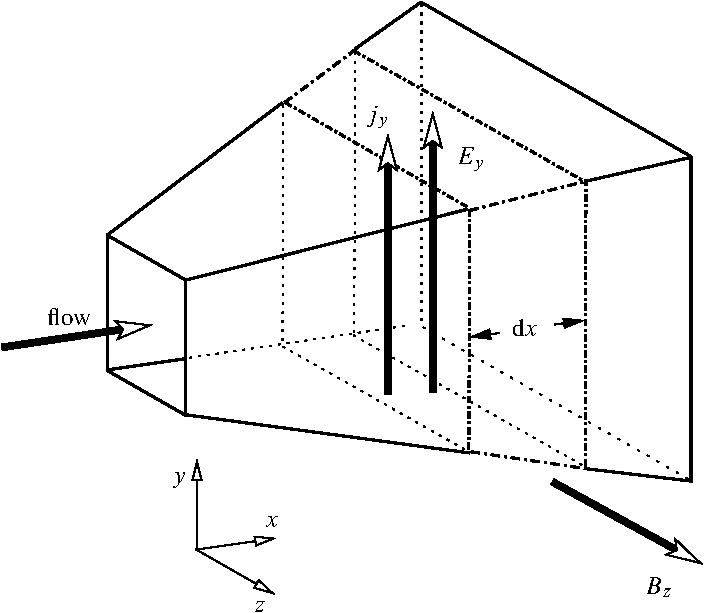
\includegraphics[width=4.0\lengthfigure]{setup.pdf}
\caption{Problem setup, showing a typical flow section with the sidewalls
         insulated and the lower and upper walls having a potential difference in the direction of
	 the current flow.}
\label{fig:setup}
\end{figure}
For a current, electric field, and magnetic field positioned as in Figure
\ref{fig:setup} we can rewrite the governing equations as:
%
\begin{equation}
  \frac{\ordi}{\ordi x}
     \left[
      \begin{array}{@{}c@{}}
        A {\rho} q \alb
        A {\rho} q^2\alb
        A {\rho} q \left(h+q^2/2\right)\alb
      \end{array}
    \right]
  +\left[
      \begin{array}{@{}c@{}}
      0 \alb
      A \ordi P / \ordi x\alb
      0 \alb
      \end{array}
   \right]
  -\left[
      \begin{array}{@{}c@{}}
      0 \alb
      A j_y B_z\alb
      A (j_y^2/\sigma + q j_y B_z)\alb
      \end{array}
   \right]=0
\end{equation}
%
Substituting the continuity equation in the momentum and energy equations, the latter
becomes:
%
\begin{eqnarray}
\frac{\ordi}{\ordi x} A \rho q &=& 0 {\rm ~~~~(continuity)}\label{eqn:continuity}\alb
  \rho q \frac{\ordi q}{\ordi x} +  \frac{\ordi P}{\ordi x} -  j_y B_z &=&0 {\rm ~~~~(momentum)}\label{eqn:momentum}\alb
  \rho q \frac{\ordi}{\ordi x} \left( h+q^2/2 \right) - (j_y^2/\sigma + q j_y B_z)&=&0 {\rm ~~~~(energy)}\label{eqn:energy}
\end{eqnarray}
%



\subsection{Increase of pressure wrt temperature}

In this subsection, we seek a relationship to find the value of $\ordi T / \ordi P$
at a specific point in the duct. Let's isolate $\ordi q / \ordi x$ in the momentum
equation, Eq.\ (\ref{eqn:momentum}), and substitute it in the energy equation, Eq.\ (\ref{eqn:energy}):
%
\begin{equation}
\rho q \frac{\ordi h}{\ordi x}
- q \frac{\ordi P}{\ordi x} + q j_y B_z
- (j_y^2/\sigma + q j_y B_z)=0~,
\end{equation}
%
and, reformatting:
%
\begin{equation}
\rho q \Cp \frac{\ordi T}{\ordi x}
- q \frac{\ordi P}{\ordi x}
- j_y^2/\sigma=0~.
\end{equation}
%
Now, let's divide each term by $q \ordi P / \ordi x$:
%
\begin{equation}
\rho \Cp \frac{\ordi T}{\ordi P}
- 1
- \frac{\ordi x }{\ordi P} \frac{j_y^2}{q\sigma}=0~,
\end{equation}
%
or,
%
\begin{equation}
\rho \Cp \frac{\ordi T}{\ordi P}
= 1
+ \frac{\ordi x }{\ordi P} \frac{j_y^2}{q\sigma}~.
\end{equation}
%
Defining the electrical load factor $K$ such that $E_y=K q B_z$, then from the generalized Ohm's
law, we get an expression for the current corresponding to $j_y=(K-1)\sigma q B_z$. Substituting
this in the latter equation yields
%
\begin{equation}
\frameeqn{
\frac{\ordi T}{\ordi P}
= \frac{1}{\rho \Cp} \left[
1
+ \frac{(K-1)^2 \sigma q B_z^2}{\ordi P / \ordi x}
\right]}~.
\label{eqn:dTdP}
\end{equation}
%
Equation (\ref{eqn:dTdP}) shows that \emph{in a compression process (\ie\ for $\ordi P / \ordi x > 0$)
the rise in temperature accompanying a rise in pressure will always be greater when
a magnetic field is present than when it is not.} In other words, whether heat is extracted or
added to the flow, whether the flow is subsonic or supersonic, the presence of a magnetic field
will \emph{always} yield a higher final static temperature for the same pressure ratio through
the compression process. Another way to look at Eq.\ (\ref{eqn:dTdP}) is by integrating both
sides on the compression/expansion path:
%
\begin{equation}
\frac{\ordi T}{T}
= \frac{R}{\Cp} \frac{\ordi P}{P}
\left[ 1 + \frac{(K-1)^2 \sigma q B_z^2}{\ordi P / \ordi x}
\right]~,
\end{equation}
%
%
or,
%
\begin{equation}
\frac{\gamma}{\gamma-1}\frac{\ordi T}{T}
=  \frac{\ordi P}{P}
+ \frac{(K-1)^2 \sigma q B_z^2}{P} \ordi x~,
\end{equation}
%
Now, integrate both sides along the flow path, going from position 1 to position 2:
%
\begin{equation}
\int \frac{\gamma}{\gamma-1}\frac{\ordi T}{T}
= \int \frac{\ordi P}{P}
+ \int \frac{(K-1)^2 \sigma q B_z^2}{P} \ordi x~,
\end{equation}
%
or,
%
\begin{equation}
\frac{\gamma}{\gamma-1} \ln \left( \frac{T_2}{T_1} \right)
= \ln \left( \frac{P_2}{P_1} \right) + \int_{x_1}^{x_2} \frac{(K-1)^2 \sigma q B_z^2}{P} \ordi x
\end{equation}
%
or,
%
\begin{equation}
\ln \left( \frac{T_2}{T_1} \right)
=   \frac{\gamma-1}{\gamma} \ln \left( \frac{P_2}{P_1} \right)
  + \frac{\gamma-1}{\gamma}\int_{x_1}^{x_2} \frac{(K-1)^2 \sigma q B_z^2}{P} \ordi x
\end{equation}
%
%
\begin{equation}
\frac{T_2}{T_1}
= \exp \left[  \frac{\gamma-1}{\gamma} \ln \left( \frac{P_2}{P_1} \right)
  + \frac{\gamma-1}{\gamma}\int_{x_1}^{x_2} \frac{(K-1)^2 \sigma q B_z^2}{P} \ordi x \right]
\end{equation}
%
%
\begin{equation}
\frac{T_2}{T_1}
= \exp \left[  \frac{\gamma-1}{\gamma} \ln \left( \frac{P_2}{P_1} \right) \right]
  \exp \left[ \frac{\gamma-1}{\gamma}\int_{x_1}^{x_2} \frac{(K-1)^2 \sigma q B_z^2}{P} \ordi x \right]
\end{equation}
%
%
\begin{equation}
\frameeqn{
\frac{T_2}{T_1}
= \left( \frac{P_2}{P_1} \right)^\frac{\gamma-1}{\gamma}
  \exp \left[ \frac{\gamma-1}{\gamma}\int_{x_1}^{x_2} \frac{(K-1)^2 \sigma q B_z^2}{P} \ordi x \right]
}
\label{eqn:T2overT1}
\end{equation}
%
Again, it can be observed that \emph{along the flow path, for a specified pressure ratio $P_2/P_1$,
the temperature ratio $T_2/T_1$ will always be higher when a magnetic field
is present.} This is due to the integral part of the second term on the RHS of
Eq.\ (\ref{eqn:T2overT1}) always yielding a positive value since all the terms except for $q$
in the integral are always positive. When $q$ is positive, then $x_2$ is consequently greater
than $x_1$, and when $q$ is negative then $x_2$ is consequently smaller than $x_1$, which \emph{always}
yields a positive integral in the end. Since the integral part of the second term is always
positive, then the second term will always be greater or equal to 1, hence always yielding a
temperature ratio greater or equal to the one obtained without any magnetic field
interaction.




%%%%%%%%%%%%%%%%%%%%%%%%%%%%%%%%%%%%%%%%%%%%%%%%%%%%%%%%%%%%%%%%%%%%%%%%%%%%%%%%%%%%%%%%%%%%%%%%%%%%%%


\section{Quasi-one-dimensional real-gas flow}

\subsection{Governing equations}

In this section, the equations governing the one-dimensional flow in a changing
cross-sectional area channel are outlined. The side walls of the channel are insulated
while the bottom and upper walls are conductors part of a closed circuit across which a
potential difference exists, as schematized in Figure \ref{fig:setup}. The magnetic field
has a component only along the $z$ coordinate (\ie\ $B_z$), while the electric field and the current
are assumed to have components only along the $y$ coordinate (\ie\ $E_y$ and $j_y$).
Then, the Euler equations in quasi-one-dimensional formulation can be written as follows:
%
\begin{equation}
 R=
      \frac{\partial {F}}{\partial X}
     -\Sda-\Smhd-\Schem~,
  \label{eqn:residual}
\end{equation}
%
where the minimization of $R$ is sought.
Due to the non-linearity of the system of equations,
a fictitious unsteady term ${\partial Q}/{\partial \pseudot}$
is necessary to obtain the right physical root from a given set of initial conditions,
\ie
%
\begin{equation}
 \frac{\partial Q}{\partial \pseudot} =-R \, .
\end{equation}
%
The vectors $Q$, $F$, and $S$ correspond to:
%
\begin{equation}
  Q=\frac{A}{J}\left[
      \begin{array}{@{}c@{}}
        {\rho}{c_1} \alb
        \vdots \alb
        {\rho}{c_\ns} \alb
        {\rho}{q} \alb
        {\rho}e+q^2/2 \alb
      \end{array}
    \right],~~~~
  F
   =A
     \left[
      \begin{array}{@{}c@{}}
        {\rho} q{c_1} \alb
        \vdots \alb
        {\rho} q{c_\ns} \alb
        {\rho} q^2 +  P\alb
        {\rho} q \left(e+q^2/2\right)+ q P \alb
      \end{array}
    \right],~~~~
  \label{eqn:S}
\end{equation}
\begin{equation}
  \Sda=\left[
      \begin{array}{@{}c@{}}
      0 \alb
      \vdots \alb
      0 \alb
      P \partial A / \partial X\alb
      0 \alb
      \end{array}
   \right],~~~~
  \Schem=
   \frac{A}{J}\left[
      \begin{array}{@{}c@{}}
      W_1 \alb
      \vdots \alb
      W_\ns \alb
      0\alb
      0\alb
      \end{array}
   \right],~~~~
  \Smhd=
   \frac{A}{J}\left[
      \begin{array}{@{}c@{}}
      0 \alb
      \vdots \alb
      0 \alb
      j_y B_z\alb
      j_y E_y \alb
      \end{array}
   \right],
\end{equation}
%
with $A$ the cross-sectional area and $J$ being the metric Jacobian, that is,
%
\begin{equation}
  J=\frac{\partial X}{\partial x}~.
  \label{eqn:J}
\end{equation}
%
For the Jachimowsky model, the chemical source term $W$ can be found, for example,
in Refs.\ \cite{thesis:1998:parent,book:1989:anderson}.
The generalized Ohm's law, neglecting the Hall effect and the ion slip, (see Ref.\
\cite{aiaabook:2001:vatazhin,book:1965:sutton}) can be written as:
%
\begin{equation}
  j_y=\sigma \left( E_y - q B_z \right)~,
  \label{eqn:j}
\end{equation}
%
where the conductivity $\sigma$ is here assumed to be scalar. For a gas weakly
ionized by electron beams powered by a fraction of the energy extracted in
a MHD generator located in the inlet of a high-speed vehicle, the conductivity
is expected to be quite low. Preliminary predictions of $\sigma$ using a computational
model was performed in Ref.\ \cite{aiaa:2002:macheret}, where the maximum value
of $\sigma$ was observed to be ranging from $1.9$ to $2.4$ $\rm S/m$.

For this paper, the thermal equation of state is assumed to be ideal, taking the form
%
\begin{equation}
  P=\sum_{k=1}^\ns \rho c_k R_k T~,
  \label{eqn:NS_state}
\end{equation}
%
while the caloric equation of state assumes a dependance of the enthalpy on
the flow temperature only, with the polynomial coefficients $a_{i,j}$
taken from McBride \cite{nasa:1993:mcbride}
%
\begin{equation}
  h_k = R_k \left( a_{1,k} T + \frac{a_{2,k}}{2} T^2 + \frac{a_{3,k}}{3} T^3
                  + \frac{a_{4,k}}{4} T^4 +\frac{a_{5,k}}{5} T^5 + a_{6,k}\right)~.
  \label{eqn:NS_caloric_state}
\end{equation}
%
The temperature $T$ is found iteratively from the flow enthalpy, which can be
determined from the $Q$ vector in this way:
%
\begin{equation}
  e=\sum_{k=1}^\ns c_k h_k-\frac{P}{\rho}~.
  \label{eqn:e}
\end{equation}
%








\section{Magnetic field originating from a magnet}

The magnetic field originating from an electromagnet (and also from some permanent magnets
magnetized in a single direction) can be approximated by a magnetic dipole moment. The error
of such an approximation can be taken as less than approximately 2\% at a distance from
the magnet greater than 5 times the largest dimension of the magnet.

In spherical coordinates,
the magnetic field of a dipole of strength $\Bdipole$ (where $\Bdipole$ is measured
at a distance $r_{\rm ref}$ from the dipole center) can be written as
(see Section 11.3 in Ref.\ \cite{book:1985:purcell}):
%
\begin{equation}
  \vec{B}=\Bdipole\frac{r_{\rm ref}^3}{r^3} \left( 2 \cos (\theta) \vec{i}_r +\sin (\theta) \vec{i}_\theta  \right)
\end{equation}
%
where $\theta$ is measured from the axis of symmetry of the dipole and where $r$ is the distance
from the center of the dipole. Also, $\vec{i}_\theta$ is a unit vector in the $\theta$
direction and $\vec{i}_r$ is a unit vector in the radial direction. The vectors
$\vec{i}_\theta$ and $\vec{i}_r$ both lie in the plane formed by the point in space
where the vectors are determined (say point {$\vec{P}$}) and two points lying on
the dipole axis of symmetry (with point {$\vec{A}$} at the dipole center and point {$ \vec{B}$}
a distance $r_{\rm ref}$ from point {$ \vec{A}$}). We can determine $\vec{i}_r$ by normalizing
the vector joining point {$\vec{A}$} and point {$\vec{P}$}:
%
\begin{equation}
\vec{i}_r=\frac{\vec{P}-\vec{A}}{|\vec{P}-\vec{A}|}
\end{equation}
%
\begin{table}[ht]
\fontsizetable
\begin{center}
  \begin{threeparttable}
    \tablecaption{$\epsilon$ and $\sigma$ for some species \tnote{1}}
    \fontsizetable
    \begin{tabular}{lllll}
      \toprule
species$_k$     &  ${\rm He}$    &  ${\rm H}_2$   &  ${\rm O}_2$   &  ${\rm N}_2$  \\
\midrule
$\epsilon_k$ [K]&  $10.22$       &  $59.7$        &  $106.7$       &  $71.4$       \\
$\sigma_k$ [nm] &  $0.2576$      &  $0.2827$      &  $0.3467$      &  $0.3798$     \\
      \bottomrule
    \end{tabular}
    \label{table:species-epssig}
    \begin{tablenotes}
      \item [1] taken from Dixon-Lewis; $T^\star_k=T/ \epsilon_k$
    \end{tablenotes}
  \end{threeparttable}
\end{center}
\end{table}
%
%
\begin{figure}
   \center
   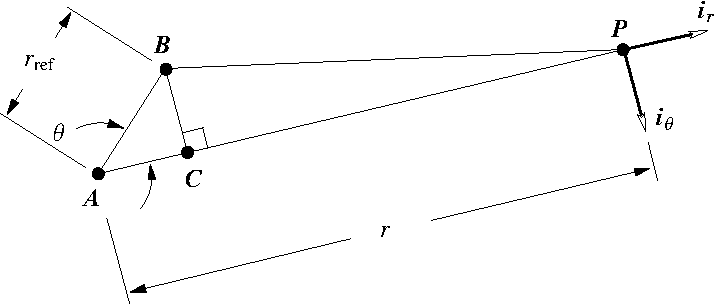
\includegraphics[width=4.0\lengthfigure]{dipoleplane.pdf}
\caption{Plane composed of the point where the magnetic field is measured (point ${\vec{P}}$)
         and two points on the dipole axis of symmetry (points $\vec{{A}}$ and ${\vec{B}}$).}
\label{fig:dipoleplane}
\end{figure}
%
and $\vec{i}_\theta$ by normalizing
the vector joining point {$ \vec{B}$} to point {$ \vec{C}$} (see Fig.\ \ref{fig:dipoleplane}).
%
\begin{equation}
\vec{i}_\theta=\frac{\vec{C}-\vec{B}}{|\vec{C}-\vec{B}|}
\end{equation}
%

\appendix
\section{Test Appendix}

where the point $\vec{C}$ corresponds to:
%
\begin{equation}
\vec{C}=r_{\rm ref} \cos \left( \theta \right) \vec{i}_r + \vec{A}
\end{equation}
%
In the above, the angle $\theta$ can be found from the law of the cosines, \ie\
%
\begin{equation}
     \cos \left( \theta \right)=
       \frac{-|\vec{B}-\vec{P}|^2 + |\vec{A}-\vec{P}|^2 + r_{\rm ref}^2}{2 r_{\rm ref}|\vec{A}-\vec{P}|}
\end{equation}
%




\bibliographystyle{waflreport}
\bibliography{all}

\end{document}










